\chapter {Design of OGM library}

We should now have all information we need to propose our solution for OGM using the \CS\ language and .NET framework.
Before we start designing individual pieces of the library, we need to define a list of requirements that should the library meet.

The solution should be able to:
\begin{itemize}
    \item {connect to a database}
    \item {map objects into graph structure}
    \item {map LINQ query into Cypher query}
    \item {execute a command in a database}
    \item {retrieve a result from the database}
    \item {map the result from the database into objects}
\end{itemize}

With these minimal requirements set, we can now go through them, analyze them, and design individual solutions for them.

\section{Connect to a database}

Neo4j company has created a client for .NET that supports both "bolt" and "neo4j" URI schemes. \cite{neo4j_client_nodate}
This driver is a NuGet package, publicly accessible and licensed under Apache 2.0 license.
This means we can use this driver in our library as a dependency.

The library should handle the driver's lifecycle.
During startup, the application should create an instance of the driver and then correctly destroy this instance on exit.

In the figure \ref{fig:components} is a visualisation of connections between components.

\begin{figure}[H]
    \centering
    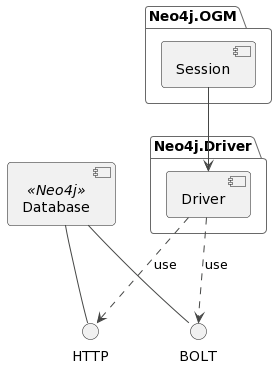
\includegraphics[width=0.4\textwidth]{content/components.png}
    \caption{Components diagram}
    \label{fig:components}
\end{figure}

We will use Neo4j's official driver for connection, but we need to encapsulate it into our library.
We will define a set of parameters for our library to ensure we have everything we need to create a connection to the database.

\section {Map objects into graph structure}

To create Cypher queries from the objects, we need to know the graph structure described in a user's domain.

What we need to do is build metadata.
To build metadata, we first need information, which assemblies contain models representing nodes and relationships in a graph.
The end-user of our library must declare these assemblies as it would be slow for our library to scan all available assemblies.

\subsection {Annotations}

To create a metadata object, we need to identify and process nodes and relationships.
We need to have a way for end-users to describe each node and its relationship with all properties they want to define.

We already have a solution to this problem, and Neo4j-\acrshort{ogm} uses it too to solve the same issue.
We will use annotations using attributes to describe nodes and their relationships.

We will look for these annotations during initialization using reflection, which is well supported by \CS\ and the .NET framework.
With annotation, we can describe the graph and create the metadata object.

\subsection {Entity mapper}

Entity mapper is a part of our library responsible for mapping entities into builders, which can be translated into Cypher queries.

For this purpose, we will define a interface \texttt{IEntityMapper}. This interface will contain
this list of public methods:

\begin{itemize}
    \item {\texttt{Map}: this method map an entity to a \texttt{ICompilerContext}}
    \item {\texttt{CompilerContext}: this method returns a current instance of\linebreak \texttt{ICompilerContext}}
\end{itemize}

In the picture \ref{fig:IEntityMapperClassDiagram} is class diagram showing entity mapper part of the library.
The interface \texttt{ICompilerContext} contains methods for controlling the context of mapped nodes and relationships.
These methods are used during mapping an entity in the \texttt{IEntityMapper.Map} method.

\begin{figure}[H]
    \centering
    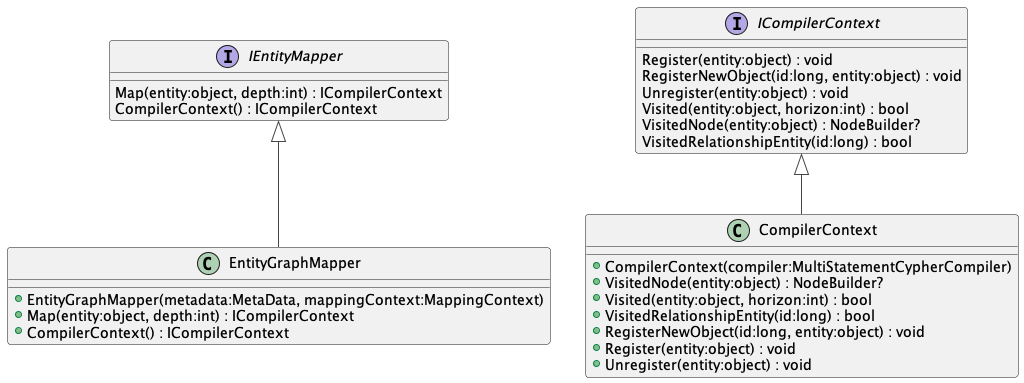
\includegraphics[width=0.8\textwidth]{content/entitymapper.png}
    \caption{\texttt{IEntityMapper} and \texttt{ICompilerContext} class diagrams}
    \label{fig:IEntityMapperClassDiagram}
\end{figure}

\section {Map LINQ query into Cypher query}

Mapping a LINQ query to a Cypher query is a bit more complicated.
As we already know, from our analysis of the Entity Framework, LINQ is translated into a custom expression tree and then into a lambda function which executes the query.
We will have to create a custom expression tree similar to the one used in the Entity Framework but optimized for Cypher language.
We can illustrate the process of transformation using the state diagram
\ref{fig:querystate}.

\begin{figure}[H]
    \centering
    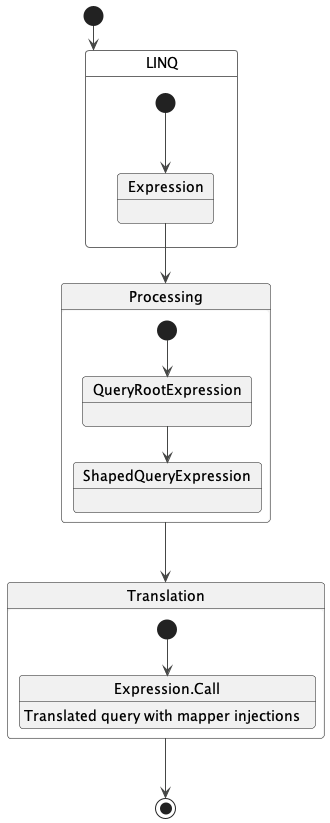
\includegraphics[width=0.5\textwidth]{content/Expression transformation.png}
    \caption{LINQ expression transformation}
    \label{fig:querystate}
\end{figure}

\subsection{\texttt{IQueryable} extension}

If we want to communicate with the database, the \texttt{IQueryable} instance must have a correct data provider.
This provider must be able to transform the expression tree into a Cypher query and enumerate the result from the database asynchronously because of the limitation of the driver.
We are going to extend \texttt{IQueryProvider} interface with \texttt{IAsyncQueryProvider} interface which declares \texttt{IAsyncQueryProvider.ExecuteAsync<T>} method.

To set a correct provider we are going to define new class that implements \texttt{IQueryable<T>} interface called \texttt{DbSet<T>}.
The name of the class is the same as it is in Entity Framework.
Besides implementing \texttt{IQueryable<T>} interface \texttt{DbSet<T>} class also implements \texttt{IAsyncEnumerable<T>} interface, because we will use asynchronous enumeration.

Because we are communicating with a database using asynchronous operations, we need to create extension methods for \texttt{DbSet<T>} which are asynchronous.
For example, LINQ has method called \texttt{FirstOrDefault} which returns first element of \texttt{IQueryable<T>} or default value of type T.
We will ahve to create an extension of \texttt{IQueryable<T>} with method \texttt{FirstOrDefaultAsync}.
This will be similar to most of the methods from LINQ.

Inside this extension method, we will call providers\linebreak\code{IAsyncQueryProvider.ExecuteAsync<T>} method.
This is our entry point, from which we will start a translation of the expression tree into a Cypher query and enumerate the result.

For better visualisation, here \ref{fig:queryprovider} is class diagram of query provider and\linebreak\texttt{DbSet<T>} class.

\begin{figure}[H]
    \centering
    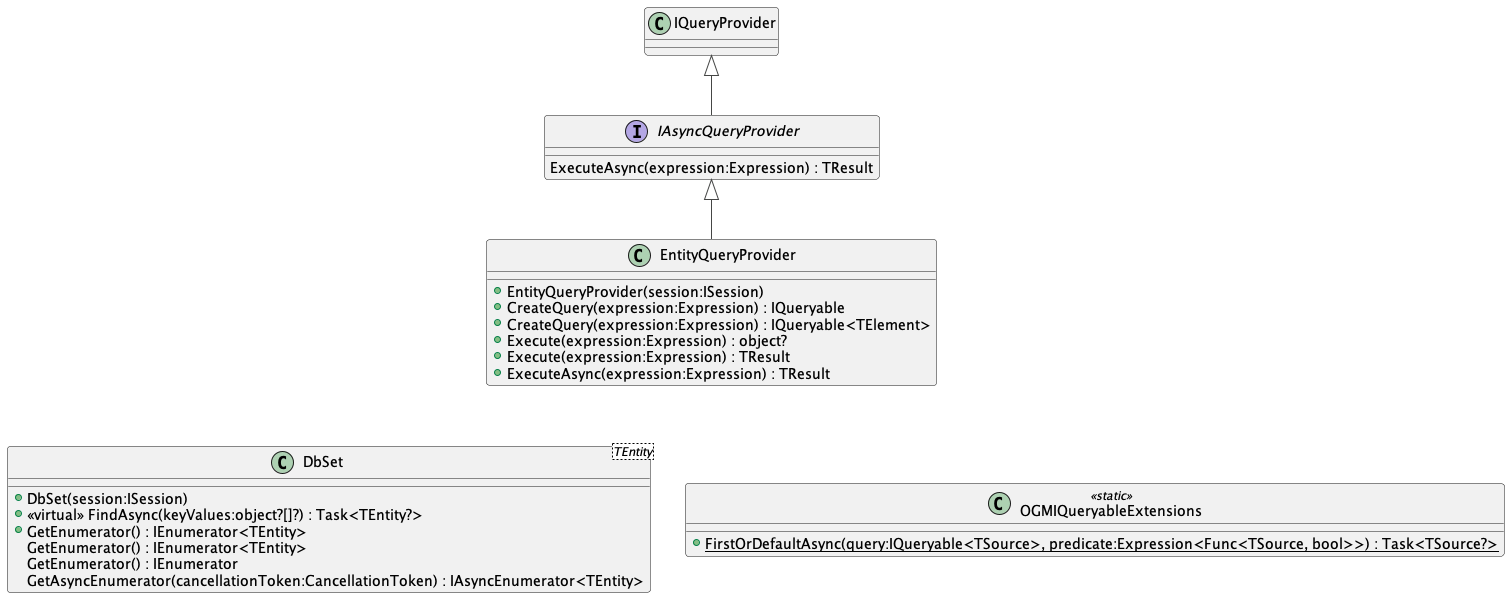
\includegraphics[width=0.9\textwidth]{content/QueryProvider.png}
    \caption{\texttt{IAsyncQueryProvider} and \texttt{DbSet<TEnity>} with extension class diagram}
    \label{fig:queryprovider}
\end{figure}

\subsection{Query compilation}

To best visualize the process of query compilation, we will use sequence diagram \ref{fig:QueryCompilerSequence}.
In this diagram, we are using different implementations of the \texttt{ExpressionVisitor} abstract class to be used in the different steps of the translation of a LINQ query into a Cypher query.

The result of this compilation will be a \texttt{Func<QueryContext, TResult>}, which is an object representing the function with the instance of the \texttt{QueryContext} class as a paramater and return object of \texttt{TResult} type.
This function does both a query execution and enumerates a result from a database response.

In the sequence diagram \ref{fig:QueryCompilerSequence}, are three expression tree visitors, each serving different purpose.
Using these visitors gives us the ability to quickly expand our library's capabilities.
We can also further expand the capabilities of defined visitors inside their implementation.

We should also introduce the concerns of each visitor. The first one that is used in the diagram is \texttt{ParameterExtractingExpressionVisitor},
which extracts parameters from the original expression.

The next one is \texttt{QueryableMethodTranslationExpressionVisitor}, this visitor will
be responsible for translating the original LINQ query into an expression tree that will be consisted of \texttt{CypherExpression} derivatives,
which will copy the Cypher language structure.

The last visitor is \texttt{ShapedQueryCompilinExpressionVisitor}, it is responsible
for taking a \texttt{ShapedQueryExpression} and translating it into a\linebreak \texttt{Expression.Call} expression, which can be then compiled into\linebreak the \texttt{Func<QueryContext, TResult>} object.

\begin{figure}[H]
    \centering
    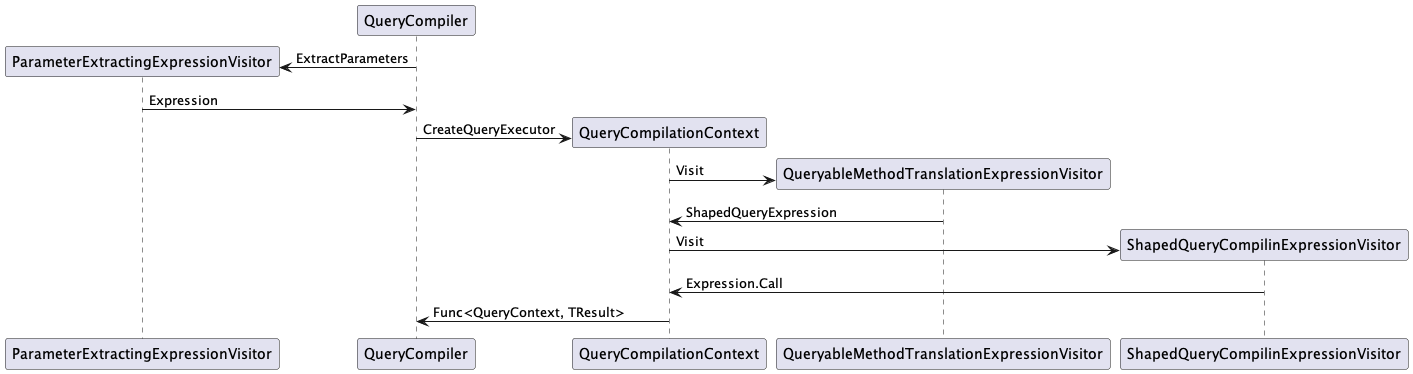
\includegraphics[width=\textheight, angle=-90]{content/Translation Sequence.png}
    \caption{\texttt{QueryCompiler} compilation sequence}
    \label{fig:QueryCompilerSequence}
\end{figure}

\section{Execute a command and retrieve the result}

We have already decided to use the official Neo4j .NET driver for communications with the database.
From this library, the result of any query is returned using the \texttt{IResultCursor} interface.
This interface is somewhat similar to an asynchronous enumerator, but it does not implement the \texttt{IAsyncEnumerable<T>} interface.
The \texttt{IResultCursor} interface declares methods as show on the \ref{fig:iresinterface} picture. We will have to adapt our code to use this interface.
We are going to use these methods inside a proper implementation of \texttt{IAsyncEnumerable<T>} interface.

\begin{figure}[H]
    \centering
    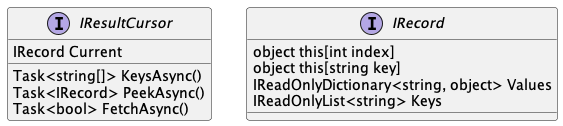
\includegraphics[width=0.7\textwidth]{content/IResultCursor.png}
    \caption{\texttt{IResultCursor} and \texttt{IRecord} interfaces}
    \label{fig:iresinterface}
\end{figure}

\section{Map the result of the query to an object}

Mapping the result into an object is our last step.
We already know from \ref{fig:iresinterface} class diagram, that we can access an \texttt{IRecord} interface using\linebreak \texttt{IResultCursor.Current} property.
This interface represents a single result of the query, which is defined in Cypher using the \texttt{RETURN} clause.

Our mapper needs to read the result and correctly choose the right key from the values.
IRecord is not a representation of a single node or relationship, but it is a representation of the \texttt{RETURN} clause, meaning that it contains all the values of the \texttt{RETURN} clause.
Mapper needs to know which key contains which entity and or value.

We can solve this issue by creating an extension method that will extend an \texttt{IRecord} interface and accept a \texttt{string} parameter defining an alias of value.
This method will return either a value or an entity.

\section{Summary}

In this chapter, we designed a solution for an \acrshort{ogm} library in .NET with LINQ to Cypher translation.
We started with defining six critical requirements that our library must solve and then went through each one and proposed a solution for them.

We defined how we would handle creating a connection to the database using Neo4j's official driver for the .NET framework.
Then we moved on to the problem of mapping objects into graph structure using annotations and reflection.
We also proposed a solution for mapping LINQ queries to Cypher queries.
At the end of the chapter, we went over the process of executions and mapping the Cypher query and its result into objects.

With this design, we should have all that we need to successfully implement \acrshort{ogm} library for .NET with LINQ to Cypher translation.
